\chapter{Event Simluation and Object Reconstruction}\label{chapter:data-mc}
Following the readout of triggered events from the CMS detector, the reconstruction of the physics objects produced by the proton-proton collision is performed, allowing for the analysis of the underlying physical processes.
Monte Carlo (MC) simulations, which provide a detailed, precise and realistic description of the expected SM and potential BSM processes at the LHC, form an essential component of performing any analysis, allowing for the development of strategies to extract processes of interest from backgrounds and the ability to make statistical interpretations of the results, such as measuring and comparing the cross sections and other properties of a measured processes to theory or by setting limits on unobserved SM or predicted BSM processes.
The event simulation and objection reconstruction algorithms which are relevant to the single top physics search presented in this thesis are discussed in this chapter.

\section{Event Simulation}\label{sec:sim}
As MC simulation is meant to provide a realistic description of the expected SM and predicted BSM processes at the LHC, 
both accurate modelling of these processes and a detailed understanding of how physical processes interact with the CMS detector are required to produce events in the same format as raw proton-proton collision data prior to undergoing the same reconstruction process.
The simulation of events is a four stage process: generation (GEN), simulation (SIM), digitisation (DIGI) and reconstruction (RECO).

The initial GEN stage involves the use \emph{event generators} to simulate the proton-proton interactions and the resultant physics processes~\cite{Buckley:2011ms,Hoche:2014rga}.
The first stage of this is the modelling of the colliding protons and the hard scattering of their constituent partons, which involves the use Parton Distribution Functions (PDFs) to assign fractions of the protons momentum to the partons and perturbation theory to compute the matrix elements of the QCD and electroweak processes involved.
The second stage models resultant parton showers through an iterative process until the infrared cutoff scale for the shower is reached, with the remaining particles undergoing hadronisation.
The various event generators used in the production of MC samples used in this thesis are discussed in~\ref{subsec:eventGenerators}.

Following the GEN stage, the SIM stage involves passing the GEN output through a complete simulation of the CMS detector that has been with the GEANT4 program~\cite{geant4,Lefebure:1999wja}.
This process models particle interactions and decays and the propagation of particles through the detector, the effects of solenoidal field and detector material.
The DIGI stage uses the SIM output to produce the detector's electronics response, which then undergoes the same RECO process that data does, as described in~\ref{sec:reco}.

The inelastic proton-proton interactions, typically called pileup (\PU), which occur both within and adjacent to the event's bunch crossing, referred to as \emph{in-time} and \emph{out-of-time] \PU  respectively, also require modelling in simulation.
Simulated \PU however, does not adequately describe observed \PU in data.
Therefore, the reweighting of the simulated samples is required and is discussed in~\ref{}.

\subsection{Event Generators}\label{subsec:eventGenerators}
\editComment{Currently being written}
%\paragraph{aMC@NLO}
%aMC@NLO~\cite{Alwall:2014hca} is a package that simulates processes to Next-To-Leading (NLO) order through the use of tree-level and one-loop
%\paragraph{Madgraph}
%\paragraph{POWHEG}
%\paragraph{Pythia}

\section{Object Reconstruction}\label{sec:reco}
Using the readouts of all of the CMS sub-detectors, a full reconstruction of the triggered physics event is undertaken.
This process involves the \emph{Particle Flow} (PF) algorithm which combines the complementary information from each of the CMS sub-detectors, as described in Chapter~\ref{chapter:lhc-cms}, to provide an optimal reconstruction and identification of all of the stable particles present in the event~\cite{CMS:2009nxa,CMS:2010eua,CMS-PRF-14-001}.
Using these reconstructed particles, additional objects such as b-jets and missing transverse energy can also be constructed.

\subsection{Charge Particle Tracks and Primary Vertices}\label{subsec:tracksVertices}
%%% Tracks
As the charged particles produced from the proton-proton collisions traverse the silicon tracker, they interact with it and leave energy deposits known as \emph{hits}.
These hits are used to reconstruct the particles' trajectories through multiple iterations of the Combinatorial Track Finder (CTF) algorithm, which is based off combinatorial Kalman Filtering~\cite{Chatrchyan:2014fea,Fruhwirth:1987fm}.

The steps of each iteration	of the CTF algorithm are:
\begin{itemize}
\item \textbf{Seed generation:} initial track candidates are formed from two or three hits to provide a first estimate of the tracks' helix parameters.
\item \textbf{Track Finding:} A combinatorial Kalman Filter then builds a candidate by adding hits from successive layers which are compatible with the extrapolated trajectory, which is updated with the addition of each subsequent hit, taking into account the hit's position, uncertainty and material traversed.
\item \textbf{Track Fitting:} The initial estimate of a built track's parameters is improved upon with the Kalman Filter performing two passes, the first from the innermost layer outwards and the second from the outermost inwards.
This approach minimises the bias in determining and discarding which hits are incorrectly associated with the track.
\item \textbf{Track Selection:} Quality criteria, such as $\chi^{2}$, the number of layers with hits and compatibility, are used to reject \emph{fake} tracks which are not associated with a charged particle.
\end{itemize}

Up to six iterations of the CTF are performed, with selected tracks' hits removed from consideration by subsequent iterations.
Whilst initial four iterations use seeds exclusively from the pixel tracker, the last two iterations uses seeds from the strip tracker to enable a high track reconstruction efficiency for those originating outside the pixel or those which did not leave any hits in the pixel tracker.

%%%Primary vertices
The reconstructed of the tracks are subsequently used to reconstruct the positions where the proton-proton collisions occurred, known as the \emph{primary vertices}~\cite{Speer:2006mh,Chatrchyan:2014fea}.
Initially track are required to be consistent with originating promptly from the interaction region, namely having a small transverse impact parameter, a minimum number of hits in the pixel and strip trackers and a low normalised $\chi^{2}$.
Such tracks are then clustered along the z-axis at their point of closest approach to the beamspot using a deterministic annealing algorithm	~\cite{Kenneth:1998i}, with these vertex candidates being used as input to an adaptive vertex filter~\cite{Fruhwirth:2007hz} to provide 3D position fits, uncertainties and variables such as the number of degrees of freedom to discriminate against fake vertices.
Out of these resultant primary vertex candidates, the one with the greatest scalar transverse momentum is considered as the \emph{primary vertex}, with the rest being considered \PU vertices.
Displaced vertices, such as those from heavy hadrons, are reconstructed during later reconstruction stages.

\subsection{Particle Flow Algorithm}
Through combining the calorimeters' energy clusters and charged particle tracks from the tracker and muon systems, the Particle Flow algorithm is able to use all the available information from an event to reconstruct and identify all stable particles in an event with far superior results than if each sub-detector were used individually.

The initial stage of the process involves associating charged particle tracks to energy clusters in the ECAL and HCAL.
Tracks are extrapolated from the last hit in the tracker to the typical shower profiles in the calorimeters, and if the particles' expected positions in the calorimeters are within the clusters' boundaries, these elements are linked together.
These linked elements are used by the Particle Flow algorithm to sequentially reconstruct and identify PF particles, removing classified elements from further consideration, with the least ambiguous or cleanest objects reconstructed first, followed by progressively more difficult objects which can be constrained by previous ones.

This is done in the following order: 
\begin{itemize}
\item muons are reconstructed, as described in Section~\ref{subsec:muons}.
\item electrons and associated Bremsstrahlung photons and isolated photons are reconstructed, as described in Section~\ref{subsec:electrons}.
\item charged hadrons are reconstructed from the HCAL clusters which are compatible with the remaining ECAL clusters and charged particle tracks.
\item any remaining ECAL and HCAL clusters with no associated charged particle tracks are reconstructed as photons and neutral hadrons respectively.
\item a post-processing stage is undertaken to mitigate against the small probability of misidentified or reconstructed particles, usually high momentum muons, causing the appearance of a large amount of missing transverse energy being present.
\end{itemize}

\subsection{Electrons}\label{subsec:electrons}
Electrons lose a significant amount of energy before reaching the ECAL due to undergoing Bremsstrahlung in the tracker layers, which often undergoes electron pair production which in turn produces further Bremsstrahlung photons.
Given that Bremsstrahlung is a non-Gaussian process and Kalman Filters assumes solely Gaussian noise contributions, a Gaussian Sum Filter (GSF) algorithm~\cite{Adam:2003eca} is used.


 
\subsection{Muons}\label{subsec:muons}
Muons tracks are independently reconstructed in both the inner tracker, as described in Section~\ref{subsec:tracksVertices}, and the muon chambers, where local reconstruction is undertaken using a Kalman Filter to build tracks from the innermost track segments of clustered DT and CSC hits outwards using DT, CSC and RPC hits.

These two types of muon tracks are reconstructed using two methods~\cite{Chatrchyan:2012xi}:
\begin{itemize}
\item \textbf{Global Muons} are reconstructed using an ``\emph{outside-in}'' approach, where tracks in the muon chambers are extrapolated inwards towards the inner tracker where candidate tracks are searched for.
If a corresponding track is found, the hits from the best candidate in the inner tracker and the muon system are fitted using a Kalman Filter.
\item \textbf{Tracker Muons} are conversely reconstructed with an ``\emph{inside-out}'' method, where inner tracker tracks with $\pT > 0.5\GeV$ and $|p| > 2.5\GeV$ are extrapolated out to the muon system using a Kalman Filter which takes into account energy losses and multiple scattering.
\end{itemize}

Given the high track reconstruction efficiencies of both the inner track and muon chambers, $\approx 99\%$ of muons produced from the proton-proton collisions (prompt muons) are reconstructed as either a global or tracker muon, if not both.
Global and tracker muons which share the same inner tracker track are merged into a single candidate muon.

\subsection{Jets}
Due to colour confinement, quarks and gluons produced from the proton-proton hard interaction rapidly hadronise, producing a collimated shower of hadrons which are clustered and reconstructed as \emph{jets}~\cite{Salam:2009jx}.
Any jet reconstruction algorithm is required to be both \emph{infrared safe} and \emph{collinear safe}, \ie so that the emission of soft gluons and the collinear splitting of gluons, respectively, does not change the jets constructed.

The main two types of jet algorithms are iterative cone and sequential recombination algorithms~\cite{Salam:2009jx}, and whilst both varieties are supported by CMS, the latter class are typically used in the majority of analyses.
The general form of a sequential recombination algorithm is:
\begin{itemize}
\item The distance, $d_{ij}$, for every pair of particles and the distance between each particle and the beamline, $d_{iB}$, is calculated.
\item If the minimum value of $d_{ij}$ is less than $d_{iB}$, the pair of particles are recombined into a single particle, and the process starts over.
\item If the minimum value of $d_{iB}$ is less than $d_{ij}$, the particle is classified as a jet and removed from the list of particles considered, and process starts over.
\item The process continues until no particles remain.
\end{itemize}

These distance variables are defined as:

\begin{equation}
d_{ij} = min(p^{2k}_{Ti},p^{2k}_{Tj}) \frac{\Delta R^{2}_{ij}}{R^{2}} \;.
\label{eq:jetAlgo1}
\end{equation}

\begin{equation}
d_{iB} = \frac{1}{p^{2k}_{Ti}} \;.
\label{eq:jetAlgo2}
\end{equation}

where $\Delta R^{2}_{ij} = (y_{i} - y_{j})^{2} + (\phi_{i} - \phi_{j})^{2}$; k = -1, 0, 1 and R is the jet size parameter which is typically set to 0.4 for CMS analyses to provide consistency with ATLAS and as it contains hadronic showers without being sensitive to \PU.
The \emph{anti-\kt} algorithm~\cite{Cacciari:2008gp}, where k = -1, which produces cone-shaped jets is commonly used in CMS.

PF jets are produced using the \emph{anti-\kt} with R = 0.4 in conjunction with PF particles produced from all the sub-detectors.
Making use of PF jets allows a more accurate reconstruction to be undertaken than if only energy clusters from the calorimeters were used, given that jets are typically composed of 65\% charged hadrons, 25\% photons and 10\% neutral hadrons, due to the precise charged hadron measurements from the tracker and ECAL which are able to constraint the small neutral hadron contribution which relies on the relatively poor resolution HCAL.

\subsubsection{Jet Energy Corrections}
Corrections are applied to the jet energies to account for the non-uniform 

Therefore, a number of corrections are applied:

~\cite{Khachatryan:2016kdb}

\subsection{b-Jets}
Correctly determining whether or not a jet was the product of a bottom quark hadronising is incredibly important for a variety of analyses, allowing them to separate signal processes from topologically similar background processes, including top physics searches due to the top quark's branching ratio to a W boson and bottom quark being $> 99\%$.
Such identification, known as \emph{b-taggging}, exploits the fact that due b hadrons having a relatively long lifetime of $\approx 1.5 ps$~\cite{Beringer:1900zz}, they travel a measurable distance away from the primary vertex before decaying. 
These secondary vertices are exploited by the \emph{Combined Secondary Vertex version 2} (CSVv2) algorithm~\cite{Chatrchyan:2012jua,CMS:206kkf}, which uses information about displaced track and secondary vertices as input into a multilayer perceptron ~\footnote{A class of neural network} to produce a discriminator value.
The CMS B-Tag and Vertexing (BTV) Physics Object Group defines working points for this (and other) algorithm's discriminator based on the mis-identification rate.

\editComment{insert fig re. discriminator}
\begin{figure}[h]
\centering
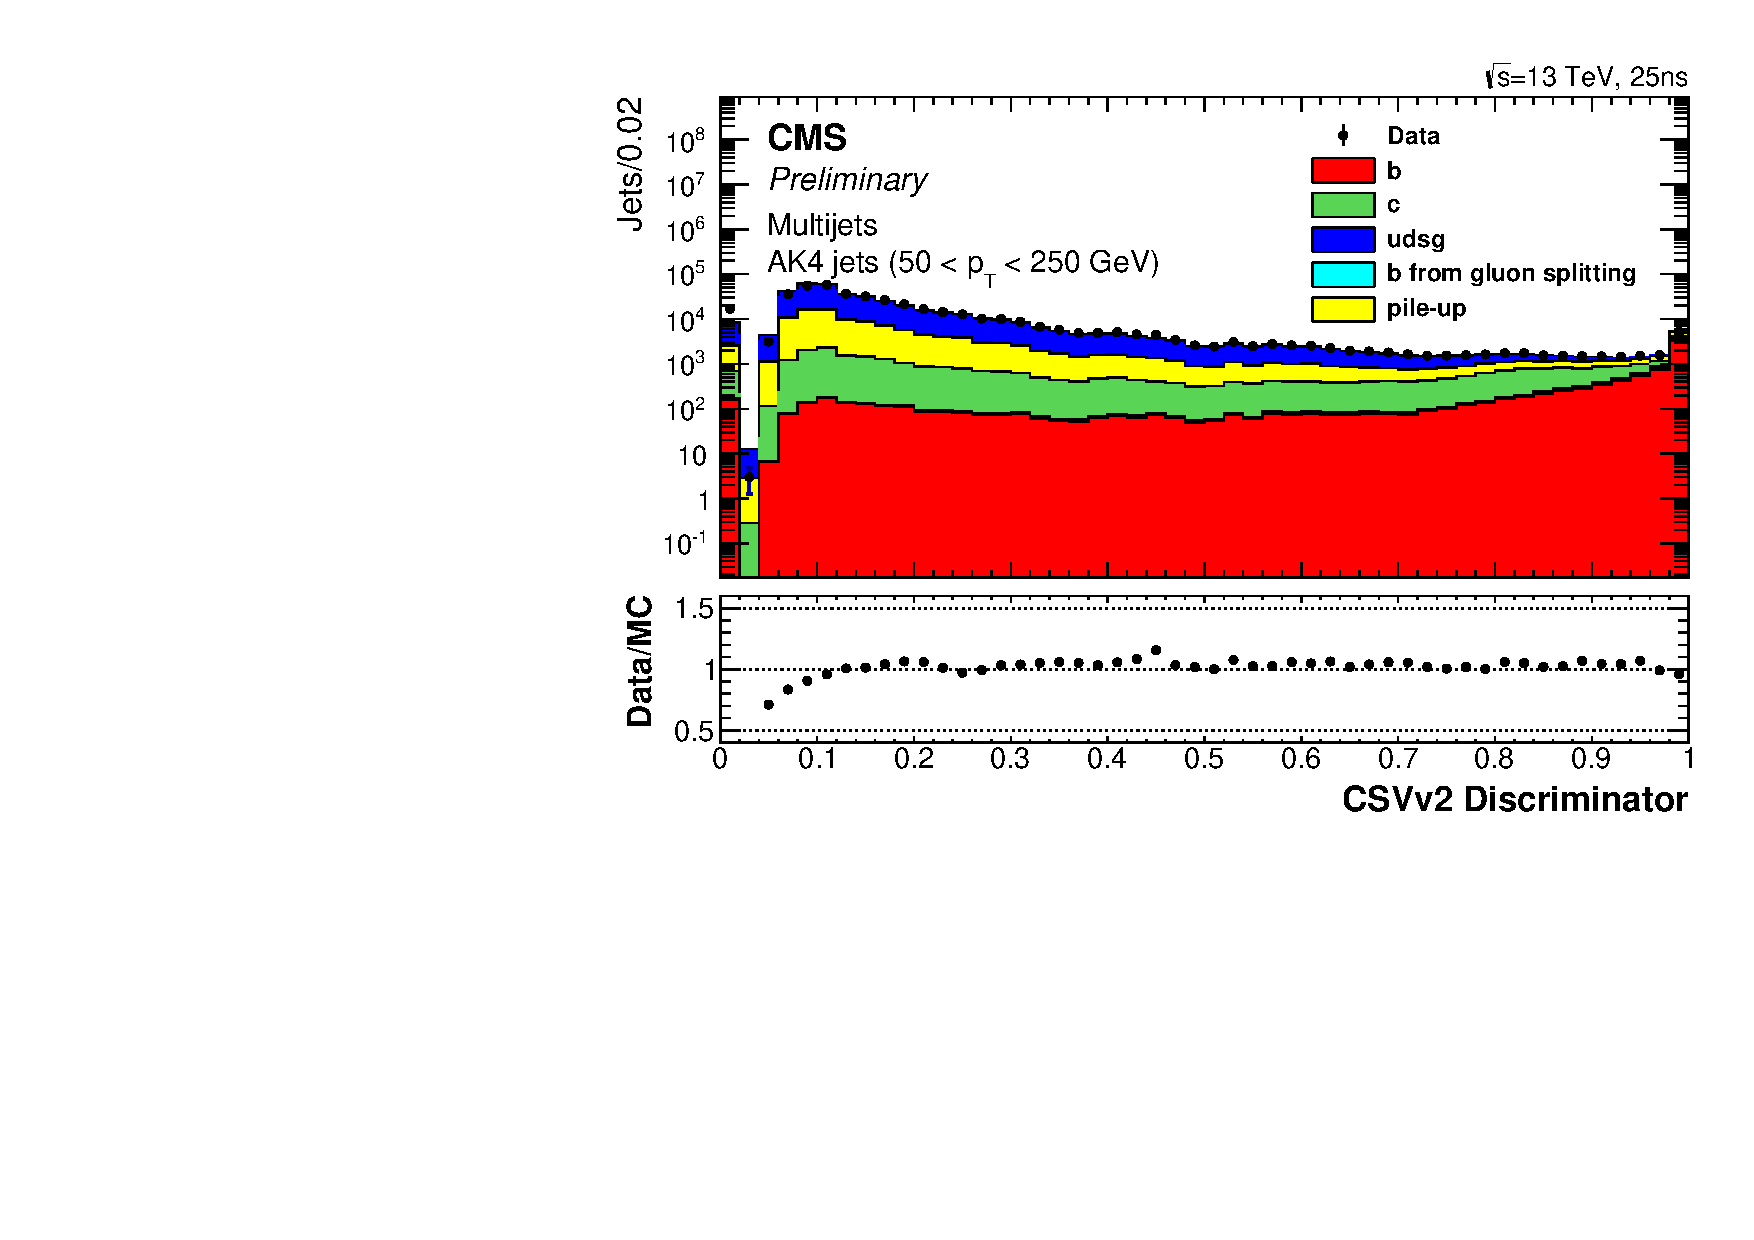
\includegraphics{figs/data-mc/ak4_pfjets_CSVIVF_Log.pdf}
\caption{The distribution of the CSVv2 algorithm's discriminator for multijet events, for $50\GeV < \pT < 250\GeV$, at \sqrt{13\TeV, where the jets have been reconstructed with the anti-\kt algorithm with R = 0.4~\cite{CMS:2016kkf}.}
\label{fig:bTagDiscriminator}
\end{figure}

\subsection{Missing Transverse Energy}
Particles which only weakly interact with matter, such as neutrinos and some hypothesised BSM particles, escape the detector without being directly observed, but can be inferred from considering the conservation of the transverse momentum of the event.
Therefore, the missing energy in the plane transverse to the beam line, \overrightarrow{\MET}, is defined as the negative vector sum of the transverse momentum in the end:

\begin{equation}
\overrightarrow{\MET} = - \sum \overrightarrow{\pT} \;.
\label{eq:MET}
\end{equation}

There are several different algorithms, using differing variables and techniques, which are used in CMS analyses to determine \MET.
PF \MET, producing using the PF particles, is used in this analysis because of its high performance with \emph{Type-I} \MET corrections applied~\cite{CMS:2016ljj}.
This correction applies the jet energy corrections discussed in~\ref{} to the PF jets with $\pT >15\GeV$ which are used in calculating the \MET.
Given that the event selection for the analysis presented in this thesis uses jets with $\pT > 30\GeV$, the \emph{Type-II} corrections (discussed in detail in~\cite{Chatrchyan:2011tn}) applied to jets with $\pT < 15\GeV$ is not considered.